\section{Introduction}\label{intro}\sloppy
\begin{itemize}
  \item exsiting data cleaning/prep fit into a pattern that is a special case of optimization
  \item what information needed to represent each special case (goal, language etc)
  \item cleaning steps >> fixes
  \item iterating over languages >> specific lceaning steps
  \item HILDA === Cleaning
  \item show how it covers most elements of data cleanig/prep/analysis pipeline.  also includes things not well supported (numbers)
  \item benefits: pefr? HILDA, optimization framework, numerics, mix and match
  \item language integration with python makes it easy to define language
\end{itemize}

Modern data scientists have vast amounts of data at their disposal from social media streams, the internet-of-things, and a growing number of open datasets.
While these new data sources are prolific, they are also substantially more variable and inconsistent than the carefully curated business data used by analysts in the past.
Consequently, every new analysis project will involve some amount of data cleaning as a first step--to resolve inconsistencies, impute missing values, and delete irrelevant data.
Data cleaning is widely reported to be one of the most time-consuming steps in the analysis process.

We can decompose data cleaning into two phases: enumeration and translation. 
In the \emph{enumeration} phase, the data scientist has to inspect the dataset to identify all of the different types of errors.
This first phase is well served by data exploration and interactive visualization tools [?].
After potential errors are identified, there is a \emph{translation} phase where the data scientist must translate those specific errors into a program composed of data transformations that can be used to clean the data.
It is the translation phase where we see the limitations of current tool, and a recent survey suggests analysts mostly use ad-hoc, single-use scripts and programs [?]. 
This practice highly problematic for reproducibility (sharing analysis between data scientists), interpretability (explaining the  data cleaning procedures),  and  scalability (extending the analyses to larger related datasets).

\begin{figure}[t]
% \vspace{-5pt}
\centering
 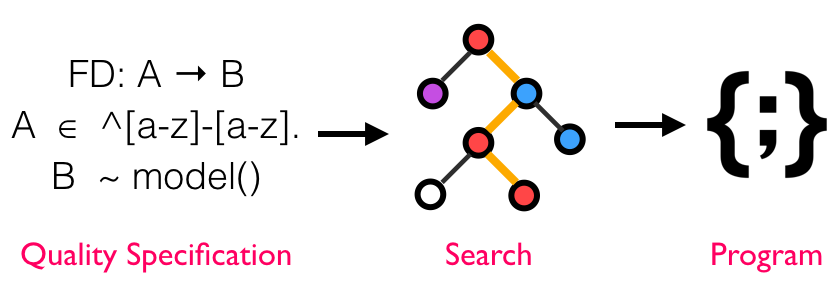
\includegraphics[width=\columnwidth]{figures/intro.png}
 \caption{ \sys is given a specification of quality (e.g., integrity constraints or a statistical model the data must conform to) and a language  of  allowed  data  transformations,  and  it  searches  to find a sequence of transformations that maximizes the quality metric. }
\end{figure}

The classical approach to addressing the translation problem is constraint-based, wherein the data scientist specifies constraints on her data in a formal language and the system searches for a satisficing database instance [?].
While there are several recent systems that apply this approach [?], one limitation is poor language integration.
For a data scientist whose project is almost entirely in Python, R, or Spark, the overhead to setting up and deploying an external cleaning systems based on a relational database can be impractical.
Furthermore, it is difficult to express domain-specific restrictions in these systems, e.g., a scientist may want to enforce that the data cleaning system handles the control group and treatment group in exactly the same way.

This paper proposes an alternative that is inspired by the constraint-based models where data cleaning is modeled as synthesizing a program that maximally satisfies some quality specification.
We present \sys, a Python library that declaratively synthesizes data cleaning programs.  \sys is given a specification of quality (e.g., integrity constraints or a statistical model the data must conform to) and a language  of  allowed  data  transformations,  and  it  searches  to find a sequence of transformations that maximizes a quality metric derived from the specification.  While the search problem is exponential in the support of the language, we apply a number of novel optimizations including:  (1) hashing to remove search branches that lead to identical results, (2) merging branches that have non-conflicting  transformations,  and  (3)  leveraging  a best-first search algorithm called SSS*.


This approach provides a number of important benefits, which we evaluate in this paper.
First, rather than editing the data in-place, \sys synthesizes a program.
This allows the cleaning operations to generalize to similar but previously unseen data.
Next, the synthesized program is represented with an intermediate representation, which can be readily transferred  between  programming languages  or  optimized  with  a compiler.
One example of an optimization is loop-fusion, where iterators over the full dataset are combined and operations are done in a single pass.









